\subsubsection{Benchmark Validation}

The first NASA sponsored ICASE/LaRC Workshop on Benchmark Problems in CAA \cite{hardin1995caaworkshop} provides an ideal point of reference for the performance of this solver. The Category 3, Problem 1 setup is designed to "...test effectiveness of radiation boundary conditions, inflow and outflow boundary conditions and the isotropy property of the computation algorithm." and specifies the linearised Euler equations to be solved with a specific set of initial conditions.

\textcite{hu1996onabsorbingbc} suggests using slightly amended pulse locations of $\left(x_1,y_1\right)=(-25,0)$ \& $\left(x_2,y_2\right)=(25,0)$ on a $-50 \leq x \leq 50$ \& $-50 \leq y \leq 50$ domain for this benchmark problem. With a standard PML width of $30\Delta x$ on all sides, Hu's locations are remapped to match the project's domain of $30 \leq x \leq 270$ \& $30 \leq y \leq 270$ at $\left(x_1,y_1\right)=(90,0)$ \& $\left(x_2,y_2\right)=(210,0)$. The solver is initiated with $M_x=0.5$, $M_y=0$, and $\sigma_{x,y}=2$ at $t=0$ using the following



\begin{equation} \label{eq:BenchmarkEqs}
    \begin{bmatrix}
    \rho \\
    u \\
    v \\
    p
    \end{bmatrix}
    = 
    \begin{bmatrix}
    1 \\
    0 \\
    0 \\
    1
    \end{bmatrix}
    % \mathrm{exp}
    e^{\left[ - \left( \mathrm{ln} \, 2 \right) \left( \frac{\left(x-x_1 \right)^2 + \left(y-y_1 \right)^2}{9} \right) \right]}
    + 
    \begin{bmatrix}
    0.1 \\
    0.04\left(y-y_2\right) \\
    -0.04\left(x-x_2\right) \\
    0
    \end{bmatrix}
    % \mathrm{exp}
    e^{\left[ - \left( \mathrm{ln} \, 2 \right) \left( \frac{ \left(x-x_2 \right)^2 + \left(y-y_2 \right)^2}{25} \right) \right]}
\end{equation}

The results of which are captured as density contours in Figure \ref{fig:Benchmark} at time snapshots from $0 \ \mathrm{s}$ to $0.75 \ \mathrm{s}$.


\begin{figure}[h!]
        \centering
        \begin{subfigure}[b]{0.475\textwidth}
            \centering
            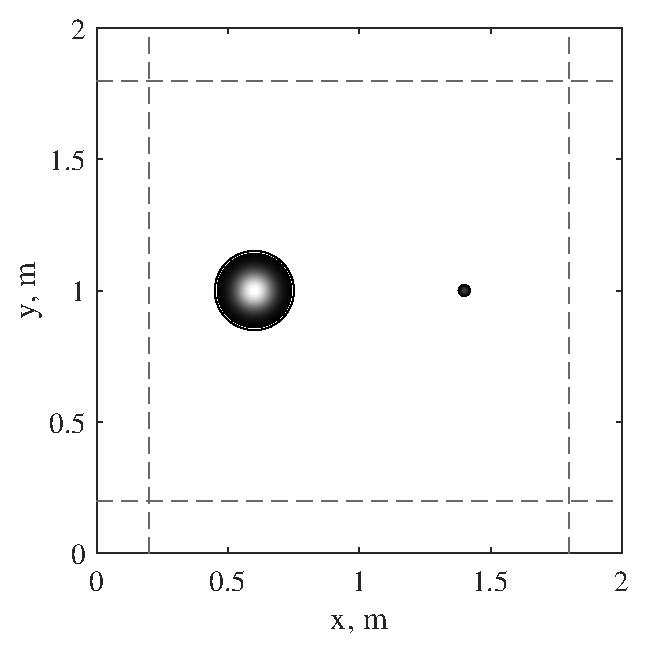
\includegraphics[width=7cm]{Figures/TechnicalAchievement/Res/Benchmark/Benchmark0.0033333s.eps}
            \caption{}    
            \label{fig:Benchmark0}
        \end{subfigure}
        \hfill
        \begin{subfigure}[b]{0.475\textwidth}  
            \centering 
            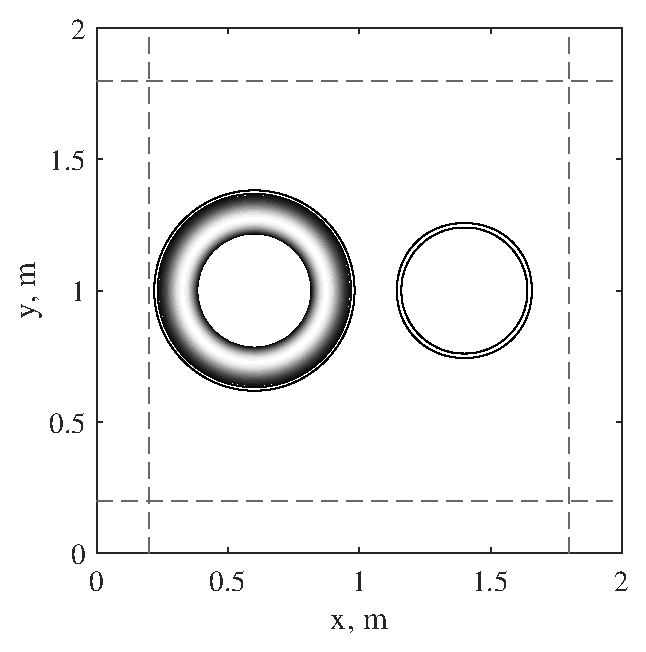
\includegraphics[width=7cm]{Figures/TechnicalAchievement/Res/Benchmark/Benchmark0.25s.eps}
            \caption{}  
            \label{fig:Benchmark025}
        \end{subfigure}
        \vskip\baselineskip
        \vspace{-0.5cm}
        \begin{subfigure}[b]{0.475\textwidth}   
            \centering 
            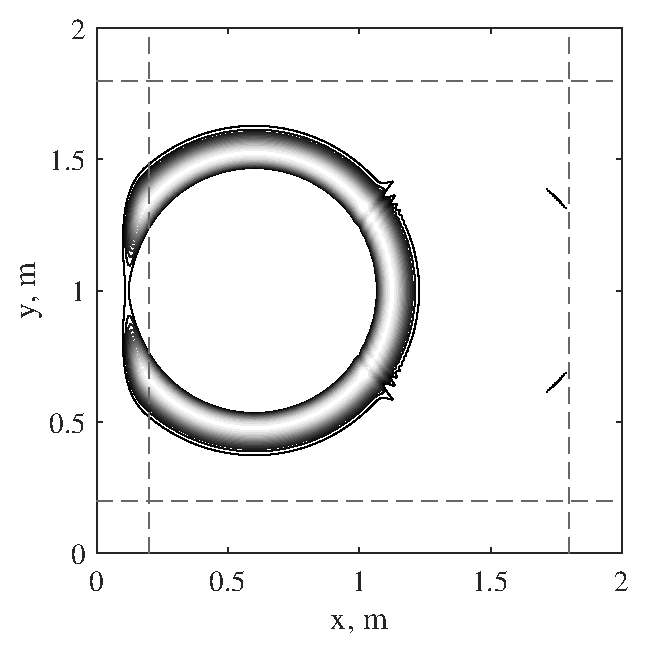
\includegraphics[width=7cm]{Figures/TechnicalAchievement/Res/Benchmark/Benchmark0.5s.eps}
            \caption{}  
            \label{fig:Benchmark05}
        \end{subfigure}
        \hfill
        \begin{subfigure}[b]{0.475\textwidth}   
            \centering 
            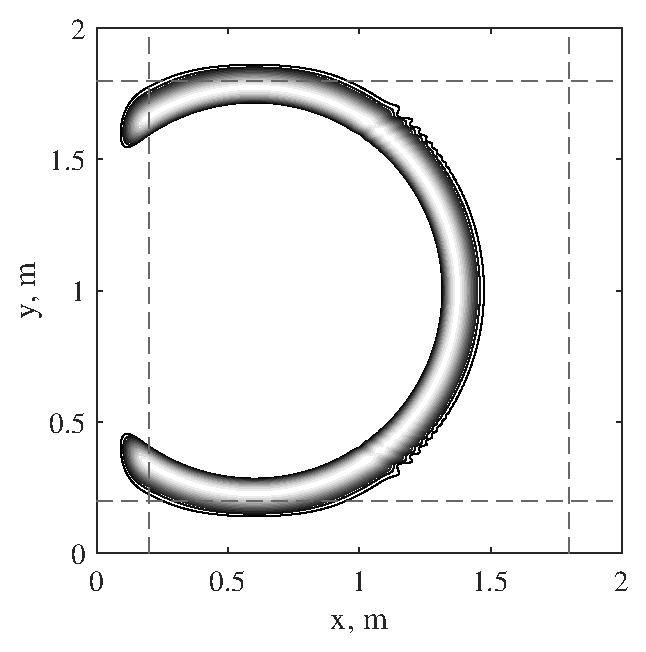
\includegraphics[width=7cm]{Figures/TechnicalAchievement/Res/Benchmark/Benchmark0.75s.eps}
            \caption{} 
            \label{fig:Benchmark075}
        \end{subfigure}
        \caption{Benchmark validation using First CAA workshop category 3 problem \cite{hardin1995caaworkshop}. Density contours ranging from $\pm0.005$ to $\pm0.1$, showing the acoustic and entropy pulses. Freestream Mach numbers set to $M_x=0.5$ and $M_y=0$, with $\sigma_x=\sigma_y=2$ and $D_x=D_y=30 \Delta x$. \textbf{(a)} $t=0 \ \mathrm{s}$, \textbf{(b)} $t=0.25 \ \mathrm{s}$, \textbf{(c)} $t=0.5 \ \mathrm{s}$, \textbf{(d)} $t=0.75 \ \mathrm{s}$.}
        \label{fig:Benchmark}
\end{figure}

When comparing the validation results to those published in \textcite{hu1996onabsorbingbc} (p.208) and \textcite{velu2010development} (p.42), the resolved wave propagation carries similar structures over time, and accurately captures the growth of the acoustic pulse - but fails to capture to magnitude and spread of the entropy pulse. Nonetheless, the solver exhibits absorption of the waves within the PML zone and demonstrates the characteristic radiation of the waves, deeming it suitable to carry out parameter optimisation.
